\subsection{Técnicas de varredura}
\label{sec:varredura}

Um dos tipos mais comuns de ataques, a varredura consiste no envio de diversos tipos de pacotes com o intuito de se conhecer mais sobre o nó alvo ou a rede em questão. Através das respostas obtidas para esses pacotes, o atacante é capaz de chegar a diversas informações que possam ajudar em futuros ataques de diversos tipos. Alguns tipos de informações que podem ser descobertas incluem (não somente): A atividade dos servidores, informações relativas a softwares utilizados no sistema, informações sobre o \textit{firewall} e topologia da rede.

Uma das principais dificuldades nas soluções desse tipo de ataque é que as varreduras são consideradas atividades legais, e ocorrem na Internet de forma rotineira, inclusive com fins não maliciosos.

Antes de explorar as técnicas de varredura, faz-se necessário o entendimento de alguns conceitos de comunicação \gls{tcp}. Para obter um serviço \gls{tcp}, uma conexão necessita ser efetivada entre os computadores origem e destino. Esta conexão é realizada através dos chamados \textit{sockets}, formados pelo par endereço \gls{ip} e número de porta, de ambos, computador de origem e computador de destino. Entre estes dois \textit{sockets} ocorre a transferência de segmentos.

Um segmento consiste em um cabeçalho \gls{tcp} seguido, opcionalmente, por informação. Um cabeçalho \gls{tcp} pode possuir seis \textit{flags} que podem ser ativadas ou desativadas ao mesmo tempo \cite{Comer:1988}, são elas:

\begin{itemize}
    \item \textbf{SYN} - \textit{bit} de sincronismo, é o \textit{bit} que informa que este é um dos dois primeiros segmentos de estabelecimento da conexão.
    \item \textbf{ACK} - \textit{bit} de reconhecimento, indica que o valor do campo de reconhecimento está carregando um reconhecimento válido.
    \item \textbf{PSH} - \textit{bit} de \textit{push}, este mecanismo, que pode ser acionado pela aplicação, informa ao \gls{tcp} origem e destino que a aplicação solicita a transmissão rápida dos dados enviados, mesmo que ela contenha um número baixo de \textit{bytes}, não preenchendo o tamanho mínimo do \textit{buffer} de transmissão.
    \item \textbf{RST} - \textit{bit} de \textit{reset}, informa o destino que a conexão foi abortada neste sentido pela origem
    \item \textbf{FIN} - \textit{bit} de terminação, indica que este pacote é um dos pacotes de finalização da conexão.
\end{itemize}

Em uma comunicação \gls{tcp}, uma conexão deve ser estabelecida entre os dois pontos (\textit{sockets}) para que a transferência de dados ocorra.
Inicialmente a máquina emissora, também chamada de cliente, transmite um segmento cuja \textit{flag} SYN é de 1 (para assinalar que se trata de um segmento de sincronização), com um número de ordem X, que se chama número de ordem inicial do cliente.

A seguir, a máquina receptora, chamada de servidor, recebe o segmento inicial que provém do cliente e envia-lhe um aviso de recepção, isto é, um segmento cuja \textit{flag} ACK é de 1 e a \textit{flag} SYN é de 1 (porque ainda se trata de uma sincronização). Este segmento contém o número de ordem do servidor, que é o número de ordem inicial do cliente. O campo mais importante deste segmento é o campo de aviso de recepção, que contém o número de ordem inicial do cliente, incrementado de 1.

Por último, o cliente transmite ao servidor um aviso de recepção, ou seja, um segmento cuja \textit{flag} ACK é de 1, cuja \textit{flag} SYN é de zero (não se trata mais de um segmento de sincronização). O seu número de ordem é incrementado e o número de aviso de recepção representa o número de ordem inicial do servidor, incrementado de 1.

Depois dessa sequência de trocas (Figura \ref{fig:troca-tcp}), também chamada de \textit{handshake}, ou, aperto de mãos em português, as duas máquinas estão conectadas e a comunicação pode ser efetivada.

\begin{figure}[H]
  \centering
  \caption{Estabelecimento de conexão TCP}
  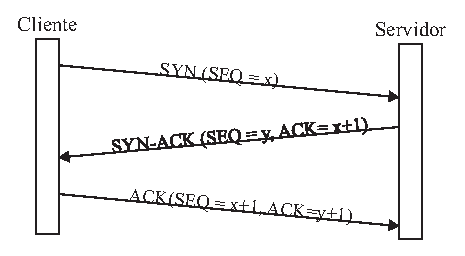
\includegraphics[width=0.5\textwidth]{images/conexao-tcp.eps}
  \label{fig:troca-tcp}
   \fonte{Elaborado pelo autor.}
\end{figure}
\FloatBarrier

Os passos a seguir são definidos pela RFC 793 \cite{rfc793}, utilizada pela grande maioria das implementações \gls{tcp} e exploradas em técnicas de varredura.

\begin{itemize}
    \item Quando um segmento SYN chega em um aporta aberta, é continuado o procedimento de \textit{handshake} como discutido anteriormente; 
    \item Quando um segmento SYN (ou FIN) chega em uma porta fechada, o segmento é descartado e um segmento RST é retornado para o cliente;
    \item Quanto um segmento FIN chega em uma porta que esteja aberta, o segmento é descartado.
    \item Quando um segmento RST chega em uma porta que esteja ouvindo (aberta), o segmento é descartado;
    \item Quando um segmento RST chega em uma porta que não esteja ouvindo (fechada), o segmento é descartado;
    \item Quando um segmento ACK chega à uma porta aberta, o mesmo é descartado e retornado um segmento RST.
\end{itemize}


Devido à sua natureza, \textit{scans} podem facilmente criar um vasto número diferente de fluxos.
Há três categorias de \textit{scans}: \textit{scan} horizontal - onde um \textit{host} varre uma porta especifica em diferentes \textit{hosts}; \textit{scan} vertical - um \textit{host} verifica várias portas em um outro \textit{host} específico; e \textit{block scan} que é a combinação dos dois \cite{Sperotto:2010}.

Existem várias técnicas de varredura de porta disponíveis e podem facilmente ser automatizadas por ferramentas como Nmap \cite{Lyon:2009}. Alguns métodos utilizados para varredura serão estudados a seguir \cite{deVivo:1999, Christopher:2001}.

\textbf{\textit{TCP Connect}} - É a forma mais comum de \textit{scanning}. Basicamente uma conexão TCP regular (\textit{handshake} completo) para cada porta definida na varredura. Para cada porta, a conexão pode resultar em sucesso, indicando uma porta aberta ou em falha caso contrário. Essa técnica é facilmente implementada pois não necessita de privilégios especiais e, do mesmo modo, é facilmente detectável. Através de \textit{logs} do sistema alvo é possível verificar mensagens de requisição de conexão e de erro para as conexões negadas. Neste método, o \textit{scanner} envia uma mensagem SYN para o sistema alvo. Se uma porta estiver (aberta) ouvindo com um serviço, a conexão se sucederá. Um SYN é retornado estabelecendo o número de sequência inicial. Um ACK considera o campo numérico de confirmação válido. Se a porta estiver (fechada) sem serviço ouvindo, uma mensagem RST é retornada, para reiniciar o pedido de conexão. Alguns exemplos de \textit{scanners} podem ser Nmap, Amap e Blaster. %Exemplo de \textit{scanner}: nmap.

\textbf{TCP SYN} - Também conhecida por \textit{Half Open} por não explorar um \textit{handshake} completo. Nesta técnica o \textit{scanner} envia uma mensagem SYN, como se estivesse pedindo uma conexão. Se responder como um RST, indica que a porta está fechada, e uma nova porta é testada. Se a resposta da máquina alvo for um SYN/ACK, indica que a porta se encontra ouvindo. O \textit{scanner} envia então um RST cancelando o \textit{handshake}. A vantagem desse tipo de \textit{scanning} é o fato de, mesmo ainda podendo ser detectado, tentativas de conexões SYN são menos frequentemente registradas se comparadas com conexões \gls{tcp} completas. %Exemplos de \textit{scanners}: amap, hping2, netstat, nmap.

\textbf{Exploração FIN} - Neste método, quando um segmento FIN é enviado para uma porta fechada, o computador alvo responde com um TCP RST. Quando a porta estiver aberta, o segmento é ignorado e o computador alvo não responde. O \textit{scanner} não recebe nunhuma resposta, pois não podem pertencer a uma conexão estabelecida. %Exemplos de \textit{scanners}: hping2, nmap.

\textbf{Xmas Tree} - é uma variação do método TCP FIN, neste, são utilizadas mensagens com prioridade TCP FIN/URG/PSH. Quando estiver ouvindo, o \textit{host} alvo não responde, caso contrário, responde com um TCP RST. %Exemplos de \textit{scanners}: hping2, netstat, nmap.

\textbf{TCP Null (sem flags ativos)} - também é uma variação do método TCP FIN, neste, tem-se resposta para portas fechadas, mas não para portas abertas.% Exemplos de \textit{scanners}: hping2, netstat, nmap.

\textbf{Varredura ACK} - Técnica utilizada para identificar \textit{firewalls}. Um segmento ACK que não pertença a nenhum conexão é gerado pelo \textit{scanner}. Se um RST é devolvido pela máquina alvo, tanto em uma porta aberta como em uma fechada, as portas são classificadas como não tendo \textit{firewall}.

\textbf{Varredura ARP} - Não se trata exatamente de varredura de portas mas essa técnica é utilizada para descobrir dispositivos ativos na rede local, para depois realizar a varredura de portas somente nos computadores ativos. O \textit{scanner} envia uma série de pacotes de protocolo \gls{arp} \cite{RFC0826} e incrementa o valor do \gls{ip} alvo a cada \textit{broadcast}.

